\documentclass[tikz,border=6pt]{standalone}
\usepackage{graphicx}
\usepackage{tikz}
\begin{document}
\begin{tikzpicture}
\definecolor{bg}{rgb}{0.04,0.05,0.09}
\fill[black] (-5.5,-5.5) rectangle (5.5,5.5);
\begin{scope}
\clip (-5.5,-5.5) rectangle (5.5,5.5);
\node at (0,0) {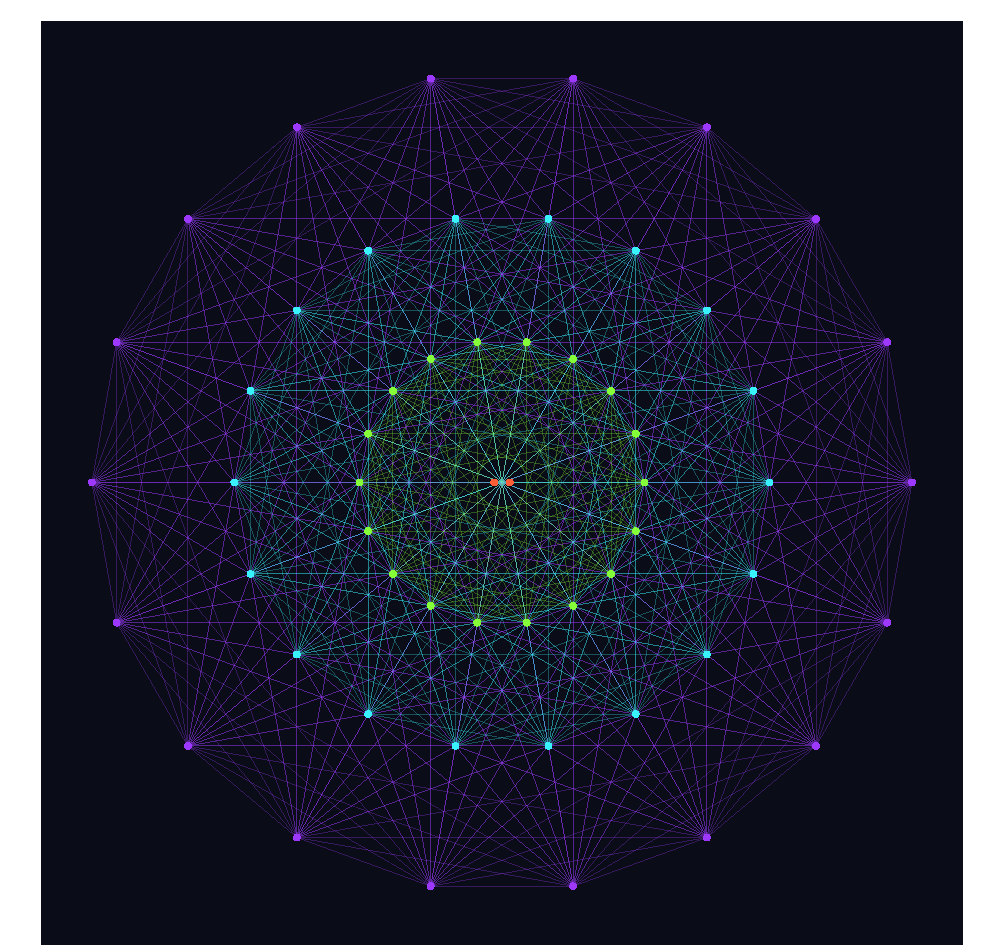
\includegraphics[width=10.0cm]{clean_e7_mandala.pdf}};
\end{scope}
\begin{scope}[shift={(-4.9,4.9)},scale=0.4]
\begin{scope}[shift={(0,0)}]
\draw[white!60!bg,line width=0.6pt] (0,0)--(1,0);
\draw[white!60!bg,line width=0.6pt] (1,0)--(2,0);
\draw[white!60!bg,line width=0.6pt] (2,0)--(3,0);
\draw[white!60!bg,line width=0.6pt] (3,0)--(4,0);
\draw[white!60!bg,line width=0.6pt] (4,0)--(5,0);
\draw[white!60!bg,line width=0.6pt] (2,0)--(2,-1);
\fill[white!90!bg] (0,0) circle (0.15);
\fill[white!90!bg] (1,0) circle (0.15);
\fill[white!90!bg] (2,0) circle (0.15);
\fill[white!90!bg] (3,0) circle (0.15);
\fill[white!90!bg] (4,0) circle (0.15);
\fill[white!90!bg] (5,0) circle (0.15);
\fill[white!90!bg] (2,-1) circle (0.15);
\end{scope}
\end{scope}
\end{tikzpicture}
\end{document}